\documentclass[11pt,fleqn]{article}

\textheight=23.3cm
\textwidth=16.5cm
\topmargin=-15mm
\oddsidemargin=0cm

\usepackage{enumerate}
\usepackage{amsmath}
\usepackage{amssymb}
\usepackage{bbm}
\usepackage{ulem}
\usepackage{graphicx}
\usepackage{wrapfig}
\usepackage{pdflscape}
\usepackage[sidewaysfigure]{rotating}
\usepackage{natbib}
\usepackage{multirow}
\newcommand{\tb}{\hspace*{3mm}}
\bibpunct{(}{)}{;}{a}{,}{,}
\parskip=3mm
\parindent=5mm
\baselineskip=17pt

\usepackage{amsthm}
\newtheorem{assumption}{Assumption}
\newtheorem{definition}{Definition}
\newtheorem{proposition}{Proposition}
\newtheorem{corollary}{Corollary}
\newtheorem{lemma}{Lemma}
\newtheorem{theorem}{Theorem}
\renewcommand{\qedsymbol}{\textit{Q.E.D.}}

\DeclareMathOperator*{\argmax}{arg\,max}
\DeclareMathOperator*{\argmin}{arg\,min}

\usepackage{hyperref}
\hypersetup{
  pdftitle={Replication of Huggett, Ventura \& Yaron (2011) - Sources of Lifetime Inequality},
  pdfauthor={Robert Kirkby},
  colorlinks=true,
  linkcolor=black,
  citecolor=black,
  urlcolor=blue,
  breaklinks=true
}


\begin{document}


%===============================
\newcommand{\rob}[1]{{\noindent\color{blue}\bf #1}}
\newcommand{\robc}[1]{{\noindent\color{blue}\bf R: #1}}
%===============================

\title{Replication of Huggett, Ventura \& Yaron (2011) - Sources of Lifetime Inequality}
\author{Robert Kirkby}
\date{\today}
\maketitle

Brief description of a replication of \cite*{HuggettVenturaYaron2011}, hereafter HVY2011. This is not intended as a full description of the model; rather, the goal is to show how the model is expressed in terms of the VFI Toolkit. For a full description see the original paper. The replication finds a better calibration than the original, but this has minimal impact on the overall results.

The replication covers all of the paper: the empirical part (the age profiles of the earnings distribution in the PSID, Fig 1, and the estimation of the human capital shocks from wage data, Table 1), the setting of model parameters including the calibration of the initial distribution (Table 2), the properties and lifetime inequality results of the benchmark model (Figs 2--5 and Tables 3, 5 and 6), the statistical models of earnings estimated on data simulated from the model (Table 4), the model with initial wealth differences (the second columns of Tables 3 and 5, and Table 6), and the sensitivity analysis of Section V.C (Fig 6, and Table \ref{tab:HVY2011_Sensitivity}). Our model reproduces the authors' model and the paper's results at the paper's parameters; our calibration fits the data better, with a higher elasticity ($\alpha=0.80$ rather than 0.70), and gives somewhat smaller roles for initial conditions (57\% rather than 61.5\% of the variance of lifetime earnings) and for learning ability. The paper's conclusions all hold. Everything is run by \verb|HuggettVenturaYaron2011.m|, including the data work and the model. The authors' replication files (PSID extracts, Matlab code for Figs 1--2, and the Fortran code for the model) are used throughout, to settle details the paper leaves open.

The replication is in some sense substantial overkill. The parameters of the initial distribution do not appear in the value function problem; they only matter for the agent distribution. HVY2011 exploit this: for each value of $\alpha$ (with $\beta$ chosen so that the capital market clears) they solve the value function once, and then estimate the initial distribution by iterating only on the agent distribution and model statistics. Since the value function is by far the most computationally costly part of the model, this massively reduces the difficulty of the problem. By contrast, the replication just uses the VFI Toolkit calibration commands, and so solves the value function at every iteration.

The rest of this document was largely written by Claude.

\section{Model description}

An agent lives from age 23 to 75, model periods $j=1,\ldots,J$ with $J=53$, and works in periods $j<J_R=39$ (ages 23--60). The state is assets $k$, human capital $h$, and learning ability $a$, which is fixed over the life cycle. A working agent splits their time between work, $l$, and learning, $s=1-l$. Earnings are $e_j=R_j h l$, where the rental rate of human capital of a cohort grows at the rate of labor-augmenting technological change, $R_j=(1+g)^{j-1}$. Human capital evolves as
\begin{align*}
 h' = \exp(z')\,H(h,s,a), \qquad H(h,s,a)=h+a(hs)^{\alpha}, \qquad z'\sim N(\mu,\sigma^2) \text{ i.i.d.}
\end{align*}
The agent solves
\begin{align*}
 V_j(k,h,a) = & \max_{c,k',l} \; u(c) + \beta\, E\left[V_{j+1}(k',h',a)\right], \qquad u(c)=\frac{c^{1-\rho}}{1-\rho}\\
 \text{subject to } & c+k' = R_j h l + (1+r) k - T_j(R_j h l, k), \qquad h' = \exp(z')H(h,1-l,a)
\end{align*}
with no debt at death. The tax system $T_j$ is a social security payroll tax of 10.6\% on earnings, a retirement transfer of 40\% of mean earnings at the end of the working life, and an income tax on earnings plus interest that follows the effective average federal income tax rates in CBO (2004). The initial condition $x_1=(h_1,a)$, with zero assets, is drawn from a bivariate log-normal distribution $\psi=LN(\mu_x,\Sigma)$.

HVY2011 compute a balanced-growth equilibrium in which factor prices are set first, $r=0.042$ and the rental rate of human capital normalized to one at age 23, and the discount factor $\beta$ is chosen so that the households' capital per unit of human capital labor equals the value implied by these prices (HVY2011 Appendix A). The parameters of $\psi$ and the elasticity $\alpha$ are chosen to minimize the sum over ages 23--60 of the squared log ratios of model to data mean earnings, variance of log earnings, and mean/median earnings (HVY2011 Appendix D). Parameter values are in Table \ref{tab:HVY2011_Table2}.


\section{VFI Toolkit implementation}

\begin{itemize}
 \item Human capital is an \emph{experience asset with an i.i.d.\ shock} (\verb|vfoptions.experienceassetu=1|): next period's $h'$ is a function of this period's decision $l$, of $h$, and of the shock $z'$, given by \verb|vfoptions.aprimeFn|. The shock is discretized with \cite{Tauchen1986} using five equally spaced points on $[\mu-2\sigma,\mu+2\sigma]$, as in HVY2011.
 \item Assets are a standard endogenous state. The grid allows borrowing (201 points on $[-1500,8000]$, including zero); together with no debt at death, the $-\infty$ return to negative consumption imposes the natural borrowing limit, which is what HVY2011 do (they relax ability-specific limits until they do not bind). Human capital is on 301 log-spaced points on $[2,4000]$, and time working on 31 points, with extra points near zero learning time (as in the authors' code). The model is solved with divide-and-conquer and a grid interpolation layer.
 \item Learning ability is a \emph{permanent type}: 11 ability levels on a grid for $\log(a)$ (discretized as normal using \cite{FarmerToda2017}). The grid depends on the mean and standard deviation of $\log(a)$, which are calibrated, so it is rebuilt at each step of the calibration using a \verb|PTypeParamFn|.
 \item The initial distribution is given as a function (\verb|jequaloneDistFn|): the bivariate log-normal on $(h_1,a)$, evaluated on the grids for human capital and ability, at zero assets. As in the authors' code, initial human capital is hit by the first shock $z_1$ before age 23, so human capital at age 23 is $\exp(z_1)h_1$. The correlation is parametrized as in Archakov \& Hansen (2021), so the correlation of the logs is $\tanh(\gamma)$ for an unrestricted $\gamma$ (restricted to $[-3,3]$).
 \item The general equilibrium has a single condition, that household $K/L$ equals the value implied by $r$, with $\beta$ as the `price', using \verb|HeteroAgentStationaryEqm_Case1_FHorz_PType|. Aggregates are for the cross-section at a point in time, so assets of age $j$ are divided by $(1+g)^{j-1}$.
 \item The calibration uses \verb|CalibrateOLGModel_PType|, with joint optimization of the calibration targets and the general equilibrium condition, calibrating $\alpha$ and the five parameters of $\psi$ (two means, two standard deviations, and the correlation). A first calibration started from HVY2011's Table 2; the final one starts from the best fit at fixed $\alpha$ found for Fig 6 (see Section \ref{sec:calibration}).
\end{itemize}

\subsection{Lifetime inequality (Table 5)}

Table 5 is the fraction of the variance of lifetime utility, $U=\sum_j\beta^{j-1}u(c_j)$, and of lifetime earnings, $X=\sum_j e_j/(1+r)^{j-1}$, due to initial conditions, $\text{Var}(E[X|x_1])/\text{Var}(X)$. Both are computed exactly, without simulation. Let $W_j(s)$ be the expected discounted sum from age $j$ given the state at age $j$, so $W_j$ is the value function for lifetime utility, and for lifetime earnings it is the value function of the policy with earnings as the return function (\verb|ValueFnFromPolicy|). Then $E[X|x_1]$ is $W_1$ evaluated at the initial condition (averaging over the shock $z_1$, as the authors' code treats $z_1$ as a shock, not an initial condition). For the total variance, the martingale $M_j=E[X|\text{age }j]$ has increments $M_j-M_{j-1}=d^{j-1}\left(W_j(s_j)-E[W_j|s_{j-1}]\right)$, where $E[W_j|s_{j-1}]=(W_{j-1}(s_{j-1})-f_{j-1}(s_{j-1}))/d$ with $d$ the discount factor and $f$ the period return, so
\begin{align*}
 \text{Var}(X) = \text{Var}_1(W_1) + \sum_{j=2}^{J} d^{2(j-1)}\left( E_j[W_j^2] - E_{j-1}\left[\left(\frac{W_{j-1}-f_{j-1}}{d}\right)^2\right]\right),
\end{align*}
where $E_j$ is the expectation over the agent distribution at age $j$, and $f_j$ is evaluated on the grid (\verb|EvalFnOnAgentDist_ValuesOnGrid_FHorz_Case1_PType|). The identity $E_j[W_j]=E_{j-1}[E[W_j|s_{j-1}]]$ holds to a relative error of at most $10^{-7}$ for earnings and $6\times10^{-5}$ for utility, in every case computed, which checks that the agent distribution, the value functions and the period returns are consistent.


\subsection{Statistical models of earnings (Table 4)}

Table 4 follows the authors' code (\verb|gmm-estimation.f| and \verb|gmm-estimation-hip.f|). In a loop of 500 iterations, each iteration simulates a panel of 200 agents followed over ages 23--60 (\verb|SimPanelValues_FHorz_Case1_PType|), adds measurement error $N(0,0.15^2)$ to log earnings, and estimates the RIP and HIP statistical models on it, by the equally weighted distance between the variances (ages 26--60) and autocovariances (one lag, `cov=1', or five lags, `cov=5') of log earnings by age and those implied by the statistical model. The statistical model, its parametrization (including the lower bounds on $\rho$ of 0.91 for RIP and 0.40 for HIP) and the initial guesses are the authors'. Table 4 reports the mean and standard deviation of the estimates across the 500 panels. [The authors instead draw 200 agents at random at each age from a single simulation of 40,000 agents, and use the AMOEBA simplex where we use \verb|fminsearch|.]

\subsection{Initial wealth differences (Tables 3, 5 and 6)}

The model with initial wealth differences follows HVY2011 Section V.A and the authors' code (\verb|hcapshocks-initw.f|, \verb|distrib-estimation-initw.f|). Initial assets are $k_1=(e^x-0.381)\,\bar{e}_{23}$, where $\bar{e}_{23}$ is mean earnings at age 23 in the data and $x\sim N(-0.277,0.921^2)$ (the PSID values in the paper; the PSID wealth data are not in the replication files), and $(\log h_1,\log a,x)$ is trivariate normal. The means and variances of $(\log h_1,\log a)$ and the three correlations are calibrated to the same earnings targets as the benchmark (with \verb|CalibrateLifeCycleModel_PType|), holding all other parameters, the prices and $\beta$ at those of the benchmark (a partial equilibrium exercise, HVY2011 footnote 25). The $3\times3$ correlation matrix is parametrized as in Archakov \& Hansen (2021). In the initial distribution, $x$ given $(\log h_1,\log a)$ is normal, so $x$ is put on 21 nodes conditional on each $(h_1,a)$ grid point, and each node's $k_1$ is put on the asset grid by linear interpolation. Lifetime wealth is lifetime earnings plus $k_1$. Table 6 is computed in this model, with the baseline at the means of $(\log h_1,\log a,x)$.

\subsection{Sensitivity (HVY2011 Section V.C)}

Four cases, each recalibrated from our calibration (with $\beta$ from the general equilibrium) and then the fractions of Table 5 computed as in the benchmark: (i) the cohort effects view of the earnings facts, recalibrating $\alpha$ and the initial distribution (the retirement transfer and the scale of the income tax use the cohort-effects mean earnings profile, which the paper does not specify); (ii) and (iii) human capital shocks with $\sigma=0.104$ and $\sigma=0.118$ (the estimate plus or minus its standard error), with $\mu$ adjusted so that the mean shock $\exp(\mu+\sigma^2/2)$ is unchanged, and $\alpha$ fixed; (iv) targeting the mean earnings profile and the age profiles of the 90--10 and 75--25 quantile ratios of earnings, with $\alpha$ fixed. For (iv) the quantile ratio profiles are computed in the data work in the same way as the other statistics (time effects), and the model's ratios are computed with \verb|CustomModelStats|, from the quantiles of earnings by age.

\section{Data}

The age profiles of Fig 1 are rebuilt from the authors' PSID extracts (1969--2004 family files, male household heads aged 23--60, with the hours and earnings restrictions of HVY2011 Section II.A), following the authors' code (\verb|Master_Figures.m|) line by line: statistics are computed for each 5-year age bin and panel year, and the age effects are estimated by regressing these on age and cohort dummies, or on age and time dummies. Our statistics by age bin and year match those saved by the authors to $10^{-11}$, and the time-effects profiles match their calibration targets to the rounding of their files. In three places the authors' code differs from the description in the paper, and we follow the code: the age bin labelled $j$ is ages $j$ to $j+4$ (the paper says centred on $j$); the mean earnings regression is in levels (the paper says logs); and the 1998, 2000 and 2002 panel years are deflated by the CPI of 1997, 1998 and 1999 (the code indexes the CPI by panel year, skipping the missing years). The smallest age-year cell has 37 observations (the paper says at least 100).

The human capital shocks (Table 1) are estimated, following the authors' code (\verb|masterfileHVY_EST.m|) and their PSID extracts, from the hourly wages (labor earnings divided by hours) of male household heads aged 55--65 (or 50--60), each followed for four years. Log hourly wages are first regressed on education and a cubic in age, and the variances and covariances of the 1, 2 and 3 year differences of the residuals, by panel year, are matched to $\text{var}(y_n)=n\sigma^2+2\sigma_\epsilon^2$ and $\text{cov}(y_n,y_m)=m\sigma^2+\sigma_\epsilon^2$ ($m<n$) by two-step GMM. After 1993 the PSID is biennial, so the later panel years have only two or three of the four years. The point estimates reproduce the authors' exactly (all ten rows, to the precision reported, with the benchmark $\sigma=0.1112$ and $\sigma_\epsilon=0.1371$ equal to the authors' output file to four decimals), as does the median number of observations per panel year. The two subperiods are of panel years (the first of the four years a panel follows people), which is what reproduces the paper's numbers of observations. Our standard errors, computed with the formula in the authors' code, are larger than the paper's by a factor of about 1.1 to 1.5 (more so the more post-1993 panel years are used), for a reason we have not found.


\section{Results}

\subsection{Calibration}\label{sec:calibration}

Our model reproduces the authors' model. At the HVY2011 Table 2 parameters the calibration objective is 0.249 in our model, against 0.264 for the authors' own model output at these parameters (which is in their replication files), with the same breakdown across the three targets (Table \ref{tab:HVY2011_Objective}), and the variance of log earnings by age is within 0.02 of theirs at every age. The general equilibrium discount factor at the Table 2 parameters is 0.9841 (HVY2011: 0.981).

However, the Table 2 parameters are not the minimum of the stated objective. A first calibration, starting from Table 2, stopped at $\alpha=0.71$ with an objective of 0.152, mostly by fitting the variance of log earnings much better. Recalibrating the initial distribution at fixed values of $\alpha$ (for Fig 6) shows that the objective is U-shaped in $\alpha$, as HVY2011 say, but with its bottom near $\alpha=0.8$ rather than 0.70: the objective is 0.269, 0.224, 0.094 and 0.121 at $\alpha=0.5,0.6,0.8,0.9$. Our calibration, starting from the $\alpha=0.8$ point, gives $\alpha=0.803$ and an objective of 0.092 (Table \ref{tab:HVY2011_Objective}); the variance of log earnings is fitted much better than at the Table 2 parameters (0.011 against 0.084), and mean earnings somewhat better (0.076 against 0.157). The discount factor, the mean, and the variance of initial human capital are close to Table 2; learning ability is less dispersed (a variance of log ability of 0.0075, against 0.012) and much less correlated with initial human capital (a correlation of logs of 0.40, against 0.81). (The first calibration, from Table 2, gave the same parameters on a coarser grid of 201 points for human capital as on the 301-point grid.) The mean earnings profile in both models is flatter than in the data (mean earnings at age 23 is about 84--87 in the model, against 72 in the data), and this accounts for most of the remaining objective.

The body of this document reports the results at our calibration. Appendix \ref{app:Table2} reports the same results at the HVY2011 Table 2 parameters, which reproduce the paper closely.

\subsection{Properties of the benchmark model and lifetime inequality}

\begin{itemize}
 \item Fit (Fig \ref{fig:HVY2011_Fig2}): the model fits the variance of log earnings, the Gini and skewness closely. Mean earnings rise less steeply than in the data, as in HVY2011.
 \item Human capital (Fig \ref{fig:HVY2011_Fig3}): 34\% of time is spent learning at age 23 (HVY2011: about 25\%), and less than 1\% after age 55. The mean human capital profile is hump shaped and flatter than the earnings profile.
 \item Risk versus ability (Fig \ref{fig:HVY2011_Fig4}): eliminating ability differences flattens the rise in dispersion, which falls over part of the working life and rises at the end; eliminating shocks gives an L-shaped dispersion profile. Both as in HVY2011.
 \item Initial distribution (Table \ref{tab:HVY2011_Table3}): human capital and learning ability are positively correlated at age 23, but less so than in HVY2011 (0.38 against 0.75), and ability is less dispersed (a coefficient of variation of 0.087, against 0.112). Mean ability is lower (0.216 against 0.329), as it must be with a higher $\alpha$.
 \item Sources of lifetime inequality (Table \ref{tab:HVY2011_Table5}): initial conditions account for 59.4\% of the variance of lifetime utility and 56.6\% of the variance of lifetime earnings, against 64.0\% and 61.5\% in HVY2011. The paper's main conclusion, that initial conditions account for more of lifetime inequality than shocks, holds at our calibration. At the Table 2 parameters our model gives 64.5\% and 61.4\% (Appendix \ref{app:Table2}). Counting the shock $z_1$ before age 23 as an initial condition would add about 3.5--4 percentage points (Table \ref{tab:HVY2011_Table5inclz1}).
 \item Initial conditions (Tables \ref{tab:HVY2011_Table6} and \ref{tab:HVY2011_Table6_benchmark}): in the model with initial wealth differences (as HVY2011 Table 6), a one standard deviation increase in initial human capital is worth 39.3\% of consumption, in learning ability 2.7\%, and in initial wealth 6.0\% (HVY2011: 39.3\%, 5.7\% and 7.1\%); in the benchmark model the first two are 41.7\% and 3.3\%. Human capital at age 23 is substantially more important than learning ability or initial wealth.
 \item Statistical models of earnings (Table \ref{tab:HVY2011_Table4}): as in HVY2011, the model's i.i.d.\ human capital shocks look highly persistent to a researcher fitting the RIP model ($\rho=0.99$; 0.98 at the Table 2 parameters; HVY2011: 0.96), and less persistent with the HIP model ($\rho=0.87$; 0.89--0.92 at the Table 2 parameters; HVY2011: 0.86). The first-order autocorrelation of earnings growth rates is $-0.37$ (HVY2011: $-0.386$), and higher orders are nearly zero, as in HVY2011. The standard deviations of the HIP estimates across panels are an order of magnitude larger than HVY2011's (0.17 against 0.010 for $\rho$). HVY2011's HIP estimates of $\rho$ (0.860 and 0.862) are within 0.003 of the value at their initial guess (0.863), and their AMOEBA simplex stops when the objective values at its vertices agree to within 0.05\%, starting from vertices very close together; this suggests their HIP estimates of $\rho$ barely move from the initial guess, which would explain the small standard deviations. Here \verb|fminsearch| is run to convergence, and $\rho$ in the HIP model is poorly identified in panels of 200 agents.
 \item Initial wealth differences (Tables \ref{tab:HVY2011_Table3}, \ref{tab:HVY2011_Table5} and \ref{tab:HVY2011_Table6}): with initial wealth, initial conditions account for 54.6\%, 56.2\% and 54.1\% of the variance of lifetime utility, earnings and wealth (HVY2011: 66.1\%, 61.3\%, 62.6\%), and a one standard deviation increase in log shifted initial wealth is worth 6.0\% of consumption (HVY2011: 7.1\%), against 39.3\% for initial human capital (HVY2011: 39.3\%) and 2.7\% for learning ability (HVY2011: 5.7\%). Unlike HVY2011, our calibrated correlations of initial wealth with initial human capital and with learning ability are negative ($-0.62$ and $-0.40$; the authors' code has 0.375 and 0.466), which is why the fractions for lifetime utility and wealth are lower than without initial wealth, where in HVY2011 they are higher. These correlations are weakly identified by the earnings targets: with borrowing up to the natural limit and no leisure, initial wealth affects earnings only through the effect of risk aversion on human capital investment, and adding initial wealth improves the fit only slightly (objective 0.085, against 0.092). Moment derivatives at our calibration (\verb|doPart(13)|; computed by central differences, as \verb|EstimateLifeCycleModel_MomentDerivatives| has no version with permanent types) confirm this. The derivatives of the 114 targeted log moments with respect to the two wealth correlations are small (norms of 1.7 and 1.1, against 6 to 21 for the means and standard deviations), and all but 0.09\% and 0.14\% of them can be reproduced by changing the other five parameters; the derivative matrix has two singular values close to zero (0.095 and 0.033, against 24.4 for the largest). Moving the wealth correlations to the authors' values raises the objective from 0.085 to 0.353 if the other parameters are held fixed, but by only 0.003 if the other parameters re-optimize (a local, Gauss--Newton, approximation): the authors' positive correlations fit essentially as well as our negative ones. At the Table 2 parameters the correlations are $-0.50$ and $0.19$, and the fractions 60.3\%, 58.8\% and 57.6\% (Appendix \ref{app:Table2}).
 \item Sensitivity (Table \ref{tab:HVY2011_Sensitivity}): all of HVY2011's conclusions hold. Smaller shocks raise the fraction of the variance of lifetime earnings due to initial conditions (62.4\% with $\sigma=0.104$) and larger shocks lower it (50.4\% with $\sigma=0.118$); targeting quantile ratios lowers it (48.4\%); and the cohort effects view gives a similar fraction (55.1\%) with a larger role for learning ability (a one standard deviation increase is worth 6.5\% of consumption, against 3.3\% in the benchmark) and a smaller role for initial human capital (37.3\%, against 41.7\%), as in HVY2011. Our fractions are 3 to 7 percentage points below HVY2011's in every case, in line with the 5 point difference in the benchmark.
 \item Consumption (Fig \ref{fig:HVY2011_Fig5}): the variance of log consumption rises by 0.09 from age 25 to 60, as in HVY2011. The data series in HVY2011 Fig 5 are taken from three other papers and are not reproduced.
 \item Elasticity parameter (Fig \ref{fig:HVY2011_Fig6}): for each $\alpha$ the initial distribution is recalibrated, and the fraction of the variance of lifetime earnings due to initial conditions is computed as for Table 5. As in HVY2011 the fraction falls as $\alpha$ rises, from 0.643 at $\alpha=0.5$ to 0.546 at $\alpha=0.9$ (HVY2011: from about 0.66 to 0.58). At $\alpha=0.9$ the variance of log ability is almost zero (0.0002).
\end{itemize}


\section{Deviations from the paper}

\begin{itemize}
 \item Details the paper leaves open follow the authors' Fortran code: the timing of the first shock (before age 23), the income tax function, the retirement transfer (0.4 times mean earnings at age 60, which is 100), the conversion of model units to dollars for the income tax (mean working-age earnings equal \$32,922), the growth of the rental rate over a cohort's life, the depreciation rate ($\delta=0.0673$, so that $K/Y=2.947$; Table 2 rounds this to 0.067), and the target $K/L$.
 \item The authors' code applies the retirees' income tax schedule at age 60 when solving the agent's problem, but the workers' schedule when simulating; we use the workers' schedule at all working ages.
 \item The authors' code hard-codes an initial distribution ($\mu_h=4.67$, $\sigma_h=0.45$, $\sigma_a=0.12$, correlation 0.78) that differs slightly from Table 2; we use Table 2.
 \item The paper's equilibrium imposes that net taxes are positive; they are (9.2 per person in the cross-section).
 \item Table 3 is computed from the log-normal distribution; HVY2011 appear to compute it from a discretized sample (their correlation of 0.746 is below the 0.782 implied by the Table 2 parameters).
 \item Lifetime inequality (Table 5) is computed exactly rather than by simulating 20,000 agents.
 \item Table 4: each of the 500 panels is 200 agents followed over all ages (the authors draw 200 agents at random at each age from one simulation of 40,000), and the statistical models are estimated by \verb|fminsearch| run to convergence (the authors use AMOEBA with a loose tolerance).
 \item Fig 6 uses $\alpha=0.5,0.6,0.8,0.9$ and our calibrated $\alpha=0.803$ (highlighted).
 \item The elasticity $\alpha$: the best fit is near 0.8, against 0.70 in HVY2011 (see the calibration discussion above).
\end{itemize}


\bibliographystyle{plainnat}
\bibliography{/home/kmarshallbanana/Dropbox/RDKbiblio.bib}


%%%%%%%%%%%%%%%%%%%%%%%%%%%%%%%%%%%%%%%%%%%%%%%%%%%
\clearpage
\section*{Tables}

\begin{table}[htp]
\caption{Table 1 of HVY2011: estimation of human capital shocks. Top: original from paper. Bottom: replication.}
\label{tab:HVY2011_Table1}
\begin{center}
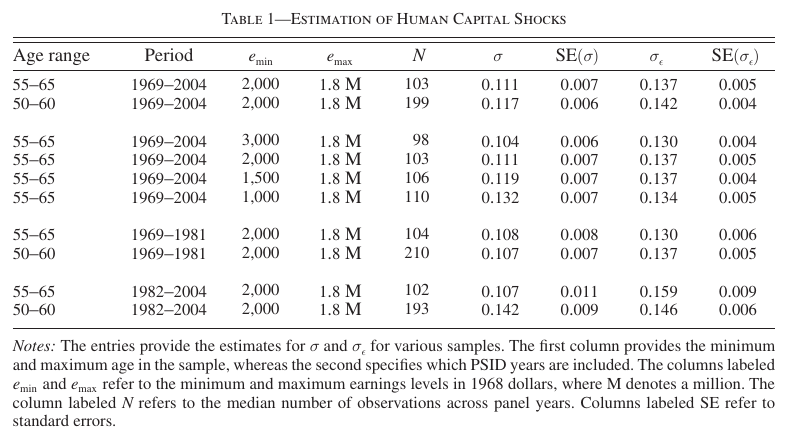
\includegraphics[width=140mm]{./OriginalTablesFigures/HVY2011_Table1.png}
\end{center}
\begin{center}
\small
\input{../SavedOutput/LatexInputs/HVY2011_Table1.tex}
\end{center}
\end{table}

\begin{table}[htp]
\caption{Table 2 of HVY2011: parameter values, benchmark model. Top: original from paper. Bottom: replication (our calibration).}
\label{tab:HVY2011_Table2}
\begin{center}
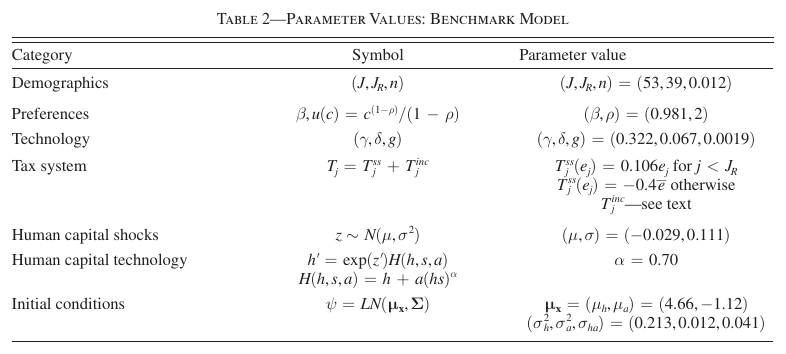
\includegraphics[width=140mm]{./OriginalTablesFigures/HVY2011_Table2.png}
\end{center}
\begin{center}
\small
\input{../SavedOutput/LatexInputs/HVY2011_Table2_calibrated.tex}
\end{center}
\end{table}

\begin{table}[htp]
\caption{The calibration objective (sum over ages 23--60 of squared log ratios of model to data moments), and its three parts. The authors' model output is their model at the Table 2 parameters, from their replication files.}
\label{tab:HVY2011_Objective}
\begin{center}
\small
\input{../SavedOutput/LatexInputs/HVY2011_Objective.tex}
\end{center}
\end{table}

\begin{table}[htp]
\caption{Table 3 of HVY2011: properties of the initial distribution. Top: original from paper. Bottom: replication (our calibration; the second column is the model with initial wealth differences).}
\label{tab:HVY2011_Table3}
\begin{center}
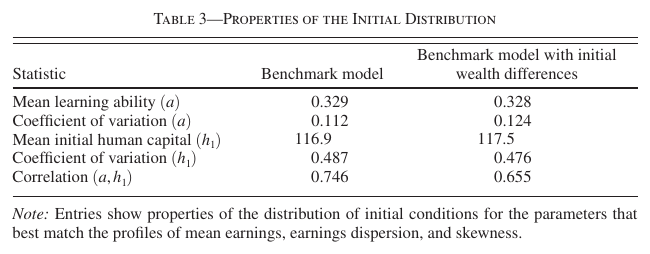
\includegraphics[width=120mm]{./OriginalTablesFigures/HVY2011_Table3.png}
\end{center}
\begin{center}
\IfFileExists{../SavedOutput/LatexInputs/HVY2011_Table3W_calibrated.tex}{\input{../SavedOutput/LatexInputs/HVY2011_Table3W_calibrated.tex}}{\input{../SavedOutput/LatexInputs/HVY2011_Table3_calibrated.tex}}
\end{center}
\end{table}

\begin{table}[htp]
\caption{Table 4 of HVY2011: statistical models of earnings, estimated on data simulated from the model (mean across 500 panels of 200 agents, standard deviation in brackets). Top: original from paper. Bottom: replication (our calibration).}
\label{tab:HVY2011_Table4}
\begin{center}
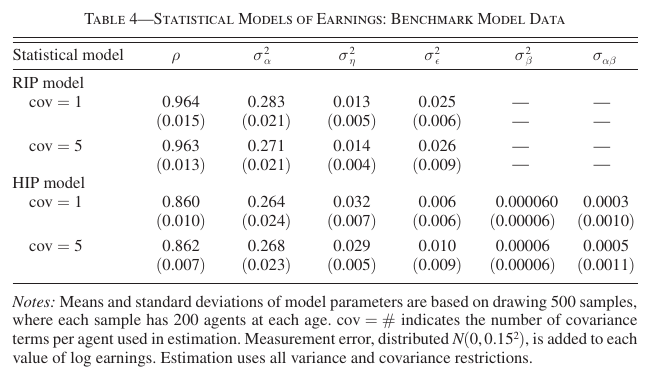
\includegraphics[width=140mm]{./OriginalTablesFigures/HVY2011_Table4.png}
\end{center}
\begin{center}
\small
\IfFileExists{../SavedOutput/LatexInputs/HVY2011_Table4_calibrated.tex}{\input{../SavedOutput/LatexInputs/HVY2011_Table4_calibrated.tex}}{\fbox{Replication to be added (doPart(10) of the replication code).}}
\end{center}
\end{table}

\begin{table}[htp]
\caption{HVY2011 Section V.C sensitivity: fraction of the variance of lifetime earnings and lifetime utility due to initial conditions, and the calibration objective (each case against its own targets). HVY2011 report these only in the text.}
\label{tab:HVY2011_Sensitivity}
\begin{center}
\small
\IfFileExists{../SavedOutput/LatexInputs/HVY2011_Sensitivity.tex}{\input{../SavedOutput/LatexInputs/HVY2011_Sensitivity.tex}}{\fbox{Replication to be added (doPart(12) of the replication code).}}
\end{center}
\end{table}

\begin{table}[htp]
\caption{Table 5 of HVY2011: sources of lifetime inequality. Top: original from paper. Bottom: replication (our calibration; the second column is the model with initial wealth differences).}
\label{tab:HVY2011_Table5}
\begin{center}
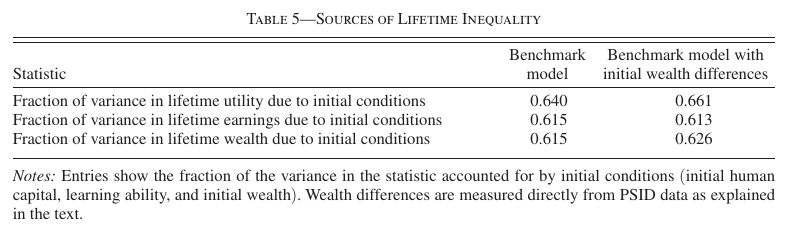
\includegraphics[width=140mm]{./OriginalTablesFigures/HVY2011_Table5.png}
\end{center}
\begin{center}
\IfFileExists{../SavedOutput/LatexInputs/HVY2011_Table5W_calibrated.tex}{\input{../SavedOutput/LatexInputs/HVY2011_Table5W_calibrated.tex}}{\input{../SavedOutput/LatexInputs/HVY2011_Table5_calibrated.tex}}
\end{center}
\end{table}

\begin{table}[htp]
\caption{Fraction of the variance due to initial conditions, if the shock $z_1$ that hits initial human capital before age 23 is counted as an initial condition. Not in HVY2011.}
\label{tab:HVY2011_Table5inclz1}
\begin{center}
\input{../SavedOutput/LatexInputs/HVY2011_Table5_inclz1.tex}
\end{center}
\end{table}

\begin{table}[htp]
\caption{Table 6 of HVY2011: changes in initial conditions. Top: original from paper. Bottom: replication (our calibration, model with initial wealth differences, baseline at the mean of the logs of initial human capital, learning ability, and shifted initial wealth).}
\label{tab:HVY2011_Table6}
\begin{center}
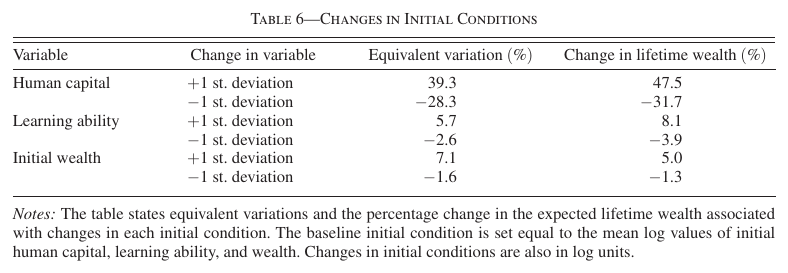
\includegraphics[width=140mm]{./OriginalTablesFigures/HVY2011_Table6.png}
\end{center}
\begin{center}
\IfFileExists{../SavedOutput/LatexInputs/HVY2011_Table6W_calibrated.tex}{\input{../SavedOutput/LatexInputs/HVY2011_Table6W_calibrated.tex}}{\input{../SavedOutput/LatexInputs/HVY2011_Table6_calibrated.tex}}
\end{center}
\end{table}

\begin{table}[htp]
\caption{Table 6 in the benchmark model (no initial wealth differences): changes in initial conditions, baseline at the mean of the logs of initial human capital and learning ability (our calibration).}
\label{tab:HVY2011_Table6_benchmark}
\begin{center}
\input{../SavedOutput/LatexInputs/HVY2011_Table6_calibrated.tex}
\end{center}
\end{table}


%%%%%%%%%%%%%%%%%%%%%%%%%%%%%%%%%%%%%%%%%%%%%%%%%%%
\clearpage
\section*{Figures}

\begin{figure}[htp]
\begin{center}
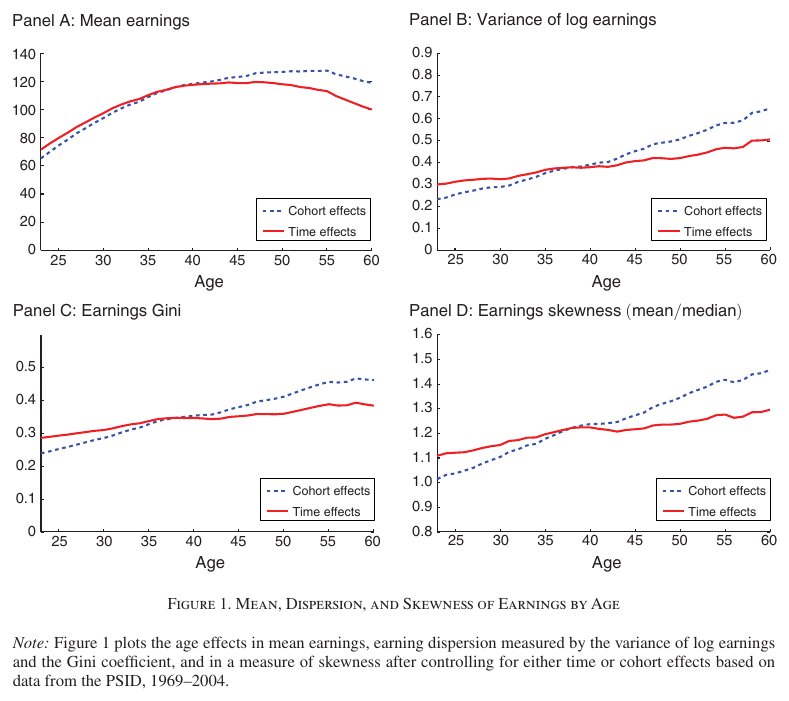
\includegraphics[width=120mm]{./OriginalTablesFigures/HVY2011_Figure1.png} \\
\includegraphics[width=120mm]{../SavedOutput/Graphs/HVY2011_Fig1.png}
\end{center}
\caption{Figure 1 of HVY2011: mean, dispersion and skewness of earnings by age, PSID data. Top: original from paper. Bottom: replication.}
\label{fig:HVY2011_Fig1}
\end{figure}

\begin{figure}[htp]
\begin{center}
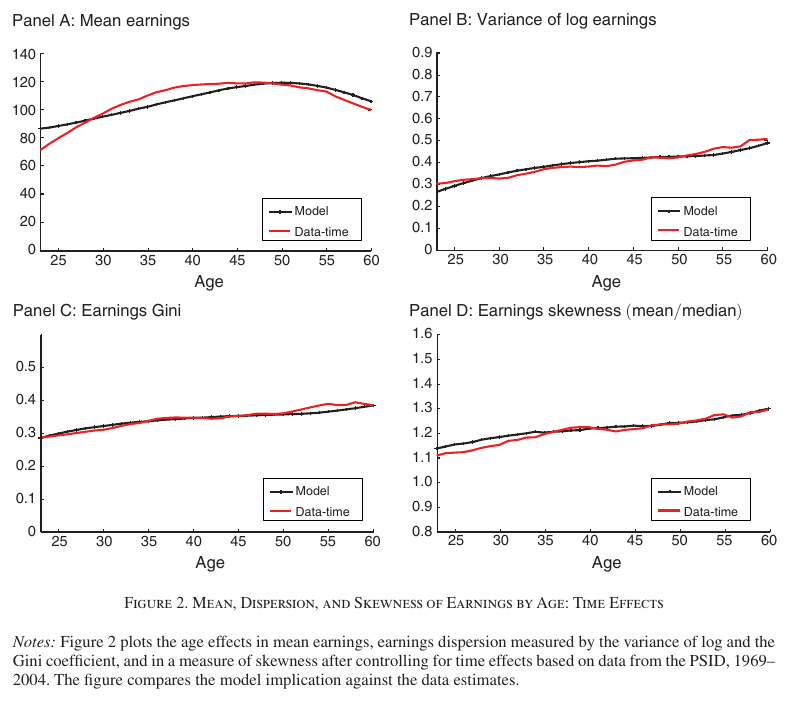
\includegraphics[width=120mm]{./OriginalTablesFigures/HVY2011_Figure2.png} \\
\includegraphics[width=120mm]{../SavedOutput/Graphs/HVY2011_Fig2_calibrated.png}
\end{center}
\caption{Figure 2 of HVY2011: mean, dispersion and skewness of earnings by age, model and data (time effects). Top: original from paper. Bottom: replication (our calibration).}
\label{fig:HVY2011_Fig2}
\end{figure}

\begin{figure}[htp]
\begin{center}
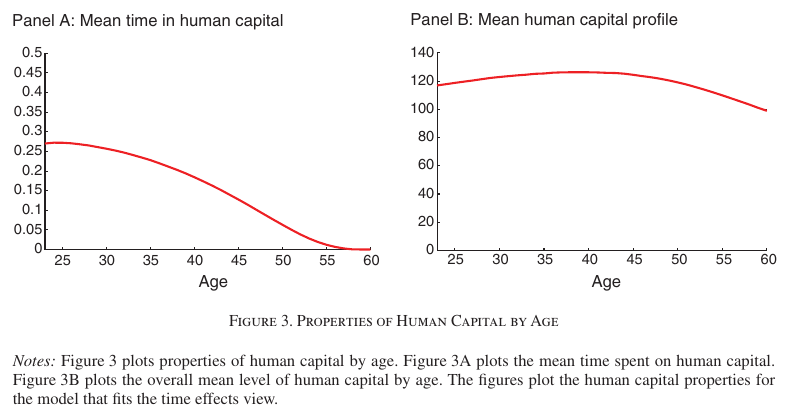
\includegraphics[width=140mm]{./OriginalTablesFigures/HVY2011_Figure3.png} \\
\includegraphics[width=140mm]{../SavedOutput/Graphs/HVY2011_Fig3_calibrated.png}
\end{center}
\caption{Figure 3 of HVY2011: properties of human capital by age. Top: original from paper. Bottom: replication (our calibration).}
\label{fig:HVY2011_Fig3}
\end{figure}

\begin{figure}[htp]
\begin{center}
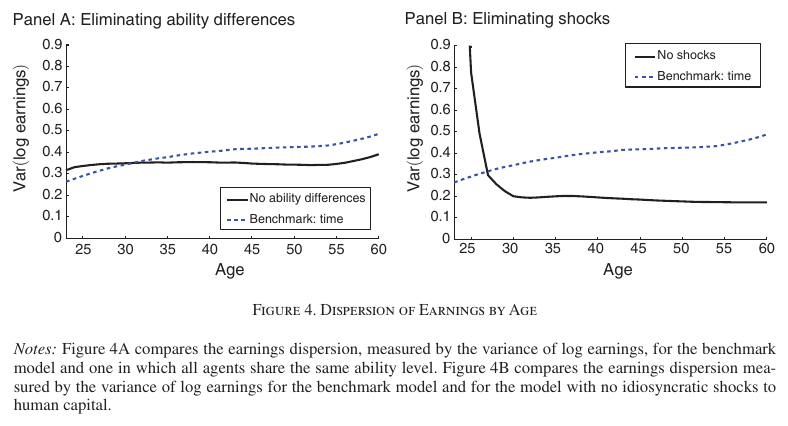
\includegraphics[width=140mm]{./OriginalTablesFigures/HVY2011_Figure4.png} \\
\includegraphics[width=140mm]{../SavedOutput/Graphs/HVY2011_Fig4_calibrated.png}
\end{center}
\caption{Figure 4 of HVY2011: dispersion of earnings by age, eliminating ability differences (Panel A) and eliminating shocks (Panel B), holding prices fixed. Top: original from paper. Bottom: replication (our calibration).}
\label{fig:HVY2011_Fig4}
\end{figure}

\begin{figure}[htp]
\begin{center}
\begin{tabular}{cc}
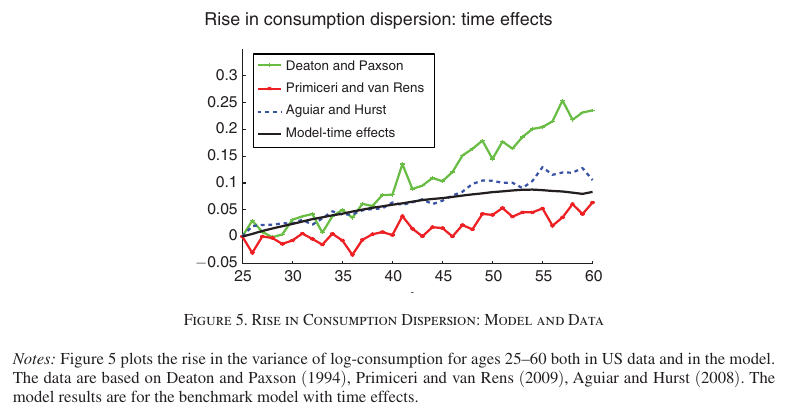
\includegraphics[width=78mm]{./OriginalTablesFigures/HVY2011_Figure5.png} & \includegraphics[width=78mm]{../SavedOutput/Graphs/HVY2011_Fig5_calibrated.png}
\end{tabular}
\end{center}
\caption{Figure 5 of HVY2011: rise in consumption dispersion (variance of log consumption relative to age 25). Left: original from paper. Right: replication (our calibration; model only, the data series are from other papers).}
\label{fig:HVY2011_Fig5}
\end{figure}

\begin{figure}[htp]
\begin{center}
\begin{tabular}{cc}
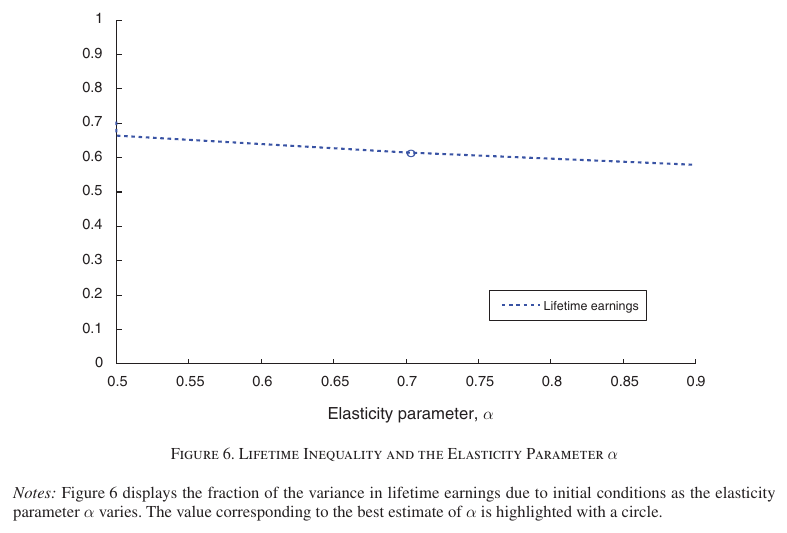
\includegraphics[width=78mm]{./OriginalTablesFigures/HVY2011_Figure6.png} &
\IfFileExists{../SavedOutput/Graphs/HVY2011_Fig6.png}{\includegraphics[width=78mm]{../SavedOutput/Graphs/HVY2011_Fig6.png}}{\fbox{\parbox{70mm}{\centering Replication to be added (doPart(7) of the replication code).}}}
\end{tabular}
\end{center}
\caption{Figure 6 of HVY2011: fraction of the variance of lifetime earnings due to initial conditions, by the elasticity parameter $\alpha$. Left: original from paper. Right: replication, recalibrating the initial distribution for each $\alpha$ (the circle is our calibration).}
\label{fig:HVY2011_Fig6}
\end{figure}


%%%%%%%%%%%%%%%%%%%%%%%%%%%%%%%%%%%%%%%%%%%%%%%%%%%
\clearpage
\appendix
\section{Results at the HVY2011 Table 2 parameters}\label{app:Table2}

This appendix reports the results of the model at the parameters of HVY2011 Table 2, with the discount factor set by the general equilibrium in our model ($\beta=0.9841$; HVY2011: 0.981). The originals are shown with the results at our calibration in the body.

\begin{table}[htp]
\caption{Parameter values at the HVY2011 Table 2 parameters (with the general equilibrium discount factor).}
\label{tab:HVY2011_Table2_table2}
\begin{center}
\small
\input{../SavedOutput/LatexInputs/HVY2011_Table2_table2.tex}
\end{center}
\end{table}

\begin{table}[htp]
\caption{Table 3 of HVY2011, at the HVY2011 Table 2 parameters: properties of the initial distribution.}
\label{tab:HVY2011_Table3_table2}
\begin{center}
\IfFileExists{../SavedOutput/LatexInputs/HVY2011_Table3W_table2.tex}{\input{../SavedOutput/LatexInputs/HVY2011_Table3W_table2.tex}}{\input{../SavedOutput/LatexInputs/HVY2011_Table3_table2.tex}}
\end{center}
\end{table}

\begin{table}[htp]
\caption{Table 4 of HVY2011, at the HVY2011 Table 2 parameters: statistical models of earnings (mean across 500 panels of 200 agents, standard deviation in brackets).}
\label{tab:HVY2011_Table4_table2}
\begin{center}
\small
\IfFileExists{../SavedOutput/LatexInputs/HVY2011_Table4_table2.tex}{\input{../SavedOutput/LatexInputs/HVY2011_Table4_table2.tex}}{\fbox{Replication to be added (doPart(10) of the replication code).}}
\end{center}
\end{table}

\begin{table}[htp]
\caption{Table 5 of HVY2011, at the HVY2011 Table 2 parameters: sources of lifetime inequality.}
\label{tab:HVY2011_Table5_table2}
\begin{center}
\IfFileExists{../SavedOutput/LatexInputs/HVY2011_Table5W_table2.tex}{\input{../SavedOutput/LatexInputs/HVY2011_Table5W_table2.tex}}{\input{../SavedOutput/LatexInputs/HVY2011_Table5_table2.tex}}
\end{center}
\end{table}

\begin{table}[htp]
\caption{Table 6 of HVY2011, at the HVY2011 Table 2 parameters: changes in initial conditions.}
\label{tab:HVY2011_Table6_table2}
\begin{center}
\IfFileExists{../SavedOutput/LatexInputs/HVY2011_Table6W_table2.tex}{\input{../SavedOutput/LatexInputs/HVY2011_Table6W_table2.tex}}{\input{../SavedOutput/LatexInputs/HVY2011_Table6_table2.tex}}
\end{center}
\end{table}

\begin{figure}[htp]
\begin{center}
\includegraphics[width=120mm]{../SavedOutput/Graphs/HVY2011_Fig2_table2.png}
\end{center}
\caption{Figure 2 of HVY2011, at the HVY2011 Table 2 parameters: mean, dispersion and skewness of earnings by age, model and data (time effects).}
\label{fig:HVY2011_Fig2_table2}
\end{figure}

\begin{figure}[htp]
\begin{center}
\includegraphics[width=140mm]{../SavedOutput/Graphs/HVY2011_Fig3_table2.png} \\
\includegraphics[width=140mm]{../SavedOutput/Graphs/HVY2011_Fig4_table2.png}
\end{center}
\caption{Figures 3 (top) and 4 (bottom) of HVY2011, at the HVY2011 Table 2 parameters: properties of human capital by age, and dispersion of earnings by age eliminating ability differences or shocks.}
\label{fig:HVY2011_Fig34_table2}
\end{figure}

\begin{figure}[htp]
\begin{center}
\includegraphics[width=90mm]{../SavedOutput/Graphs/HVY2011_Fig5_table2.png}
\end{center}
\caption{Figure 5 of HVY2011, at the HVY2011 Table 2 parameters: rise in consumption dispersion (model only).}
\label{fig:HVY2011_Fig5_table2}
\end{figure}


\end{document}
